\begin{figure}[htbp]
\centering
\resizebox{\linewidth}{!}{%
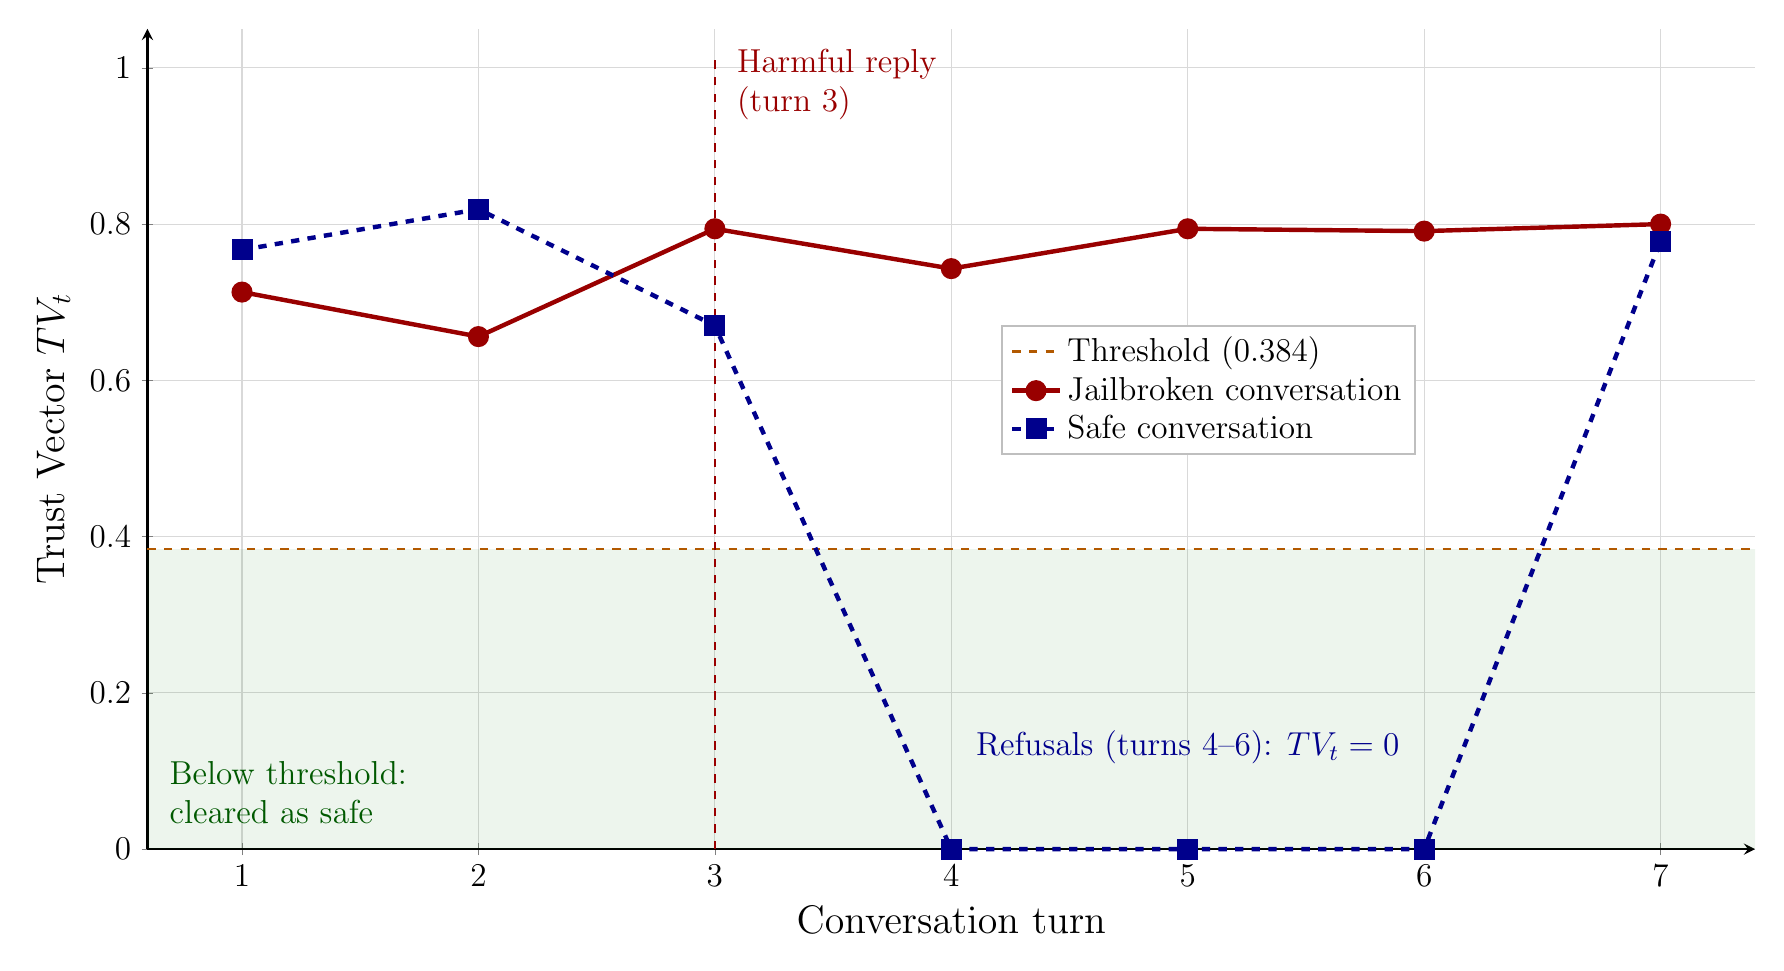
\begin{tikzpicture}[font=\sffamily]
\begin{axis}[
    width=22cm, height=12cm,
    xlabel={\Large Conversation turn},
    ylabel={\Large Trust Vector $TV_t$},
    xmin=0.6, xmax=7.4, ymin=0, ymax=1.05,
    xtick={1,2,3,4,5,6,7},
    ytick={0,0.2,0.4,0.6,0.8,1.0},
    tick label style={font=\large},
    label style={font=\large},
    axis lines=left,
    grid=major, grid style={gray!30},
    thick, clip=false,
    legend style={font=\large, draw=gray!50, fill=white, at={(0.66,0.56)}, anchor=center},
    legend cell align={left}
]
% shaded region below the threshold = cleared as safe
\addplot[draw=none, fill=green!45!black, fill opacity=0.07, forget plot] coordinates {(0.6,0) (7.4,0) (7.4,0.384) (0.6,0.384)} \closedcycle;
\addlegendimage{dashed, thick, orange!70!black}
\addlegendentry{Threshold (0.384)}
\addplot[dashed, thick, orange!70!black, forget plot] coordinates {(0.6,0.384) (7.4,0.384)};
% jailbroken conversation (locked id 22240)
\addplot[red!60!black, solid, ultra thick, mark=*, mark size=3pt, mark options={fill=red!60!black}]
    coordinates {(1,0.713) (2,0.656) (3,0.794) (4,0.743) (5,0.794) (6,0.791) (7,0.800)};
\addlegendentry{Jailbroken conversation}
% safe conversation (locked id 4579)
\addplot[blue!55!black, dashed, ultra thick, mark=square*, mark size=3pt, mark options={fill=blue!55!black, solid}]
    coordinates {(1,0.767) (2,0.819) (3,0.670) (4,0.000) (5,0.000) (6,0.000) (7,0.778)};
\addlegendentry{Safe conversation}
% annotations
\draw[dashed, thick, red!60!black] (axis cs:3,0) -- (axis cs:3,1.02);
\node[align=left, font=\large, text=red!60!black, anchor=south west] at (axis cs:3.05,0.92) {Harmful reply\\(turn 3)};
\node[align=center, font=\large, text=blue!55!black] at (axis cs:5,0.13) {Refusals (turns 4--6): $TV_t = 0$};
\node[align=left, font=\large, text=green!35!black, anchor=south west] at (axis cs:0.65,0.02) {Below threshold:\\cleared as safe};
\end{axis}
\end{tikzpicture}%
}
\caption{Trust Vector per turn for two real conversations from the locked Llama-3.1-8B-Instruct XGuard-Train set: the first jailbroken and the first safe conversation in the locked random sample that have at least five replies. The dashed line is the set's threshold at 100\% sensitivity. The jailbroken conversation stays above the threshold up to the harmful reply at turn 3; in the safe conversation the model refuses at turns 4--6 and TV falls to 0, below the threshold.}
\label{fig:tvturns}
\end{figure}
